\documentclass[11pt,a4paper]{article}

\usepackage[T1]{fontenc}
\usepackage{lmodern}
\usepackage[english]{babel}
\usepackage[margin=2.2cm]{geometry}
\usepackage{amsmath}
\usepackage[per-mode=symbol]{siunitx}
\usepackage{booktabs}
\usepackage{tabularx}
\usepackage{graphicx}
\usepackage[font=small, labelfont=bf, margin=0.5cm]{caption}
\usepackage{tikz}
\usepackage{microtype}
\usepackage{csquotes}
\usepackage[backend=biber, style=numeric-comp, sorting=none, maxbibnames=5, giveninits=true, doi=true, isbn=false, url=false]{biblatex}
\usepackage[colorlinks=true, linkcolor=blue!50!black, citecolor=blue!50!black, urlcolor=blue!50!black]{hyperref}
\usepackage[capitalise, noabbrev]{cleveref}

\addbibresource{references.bib}
\graphicspath{{figures/}}
\setlength{\parskip}{0.35em}
\setlength{\parindent}{0pt}

\newcommand{\Cu}{\mathrm{Cu}}
\newcommand{\Zn}{\mathrm{Zn}}
\newcommand{\Tc}{T_\mathrm{c}}

\hypersetup{pdftitle={Order-disorder transition of beta-brass (CuZn)}, pdfauthor={Tony Pansera, Noé Fourniol}}

\begin{document}
\begin{center}
  
\includegraphics[height=1.5cm]{logo_centralesupelec.png}\par
  \vspace{1.2em}
  {\LARGE\bfseries Order--disorder transition of $\beta$-brass (CuZn)\\[0.2em]
    by Metropolis Monte Carlo on a rigid lattice\par}
  \vspace{1.2em}
  {\large Tony Pansera \qquad Noé Fourniol\par}
  \vspace{0.6em}
  CentraleSupélec --- course \emph{Modélisation et simulation numérique}, project report\par
  \vspace{0.3em}
  November 2026\par
\end{center}

\begin{abstract}
\noindent
We wrote a Metropolis Monte Carlo code that exchanges Cu and Zn atoms on a fixed body-centred cubic lattice of 432 sites, with a pair energy model limited to first and second neighbours.
The code reproduces the exact values of the perfect B2 structure (cohesive energy \SI{2.484}{eV/atom}) and of a random alloy.
Scanning the temperature from \SIrange{200}{1600}{K}, we follow the energy, the heat capacity, the long-range order parameter $\eta$, its susceptibility and the Cowley short-range order parameters.
The three estimates of the transition temperature all give $\Tc \approx \SI{720}{K}$, close to the experimental value of about \SI{740}{K} and well below the Bragg--Williams mean-field value of \SI{894}{K}.
Short-range order survives above $\Tc$.
\end{abstract}

% =====================================================================
\section{Introduction}

$\beta$-brass is the CuZn alloy with about 50\,\% Zn.
At low temperature it is ordered in the B2 (CsCl-type) structure: the atoms sit on a body-centred cubic (bcc) lattice, Cu on the cube corners and Zn on the cube centres.
When the temperature rises, Cu and Zn atoms swap places more and more often.
Around \SI{740}{K} the distinction between the two kinds of sites disappears: the alloy becomes a disordered bcc solid solution~\cite{NixShockley1938,Massalski1990,KhanEisenbach2016}.
This is a classic order--disorder transition, first described by Bragg and Williams with a mean-field theory~\cite{BraggWilliams1934}.

In this project~\cite{Sujet2026} the atoms do not move away from the lattice sites (\enquote{rigid lattice}): only the occupation of each site by Cu or Zn changes.
The energy is a sum of pair interactions between first and second neighbours.
We sample the equilibrium configurations with the Metropolis algorithm~\cite{Metropolis1953} and measure how the order is lost when the temperature increases.

The report follows the questions of the project.
\Cref{sec:model} describes the model and the algorithm, and \cref{sec:conditions} gives all the simulation parameters.
\Cref{sec:checks} tests the program and gives the cohesive energy.
\Cref{sec:equilibration} shows how long the system takes to reach equilibrium.
\Cref{sec:results} presents the physical quantities as a function of temperature, \cref{sec:tc} the transition temperature and \cref{sec:discussion} the discussion.

% =====================================================================
\section{Model and method}
\label{sec:model}

\subsection{Lattice and neighbours}

The simulation box contains $6\times6\times6$ cubic cells of side $a$, with two sites per cell (\cref{fig:cell}): a site of sublattice $\alpha$ at the corner $(0,0,0)$ and a site of sublattice $\beta$ at the centre $(\frac12,\frac12,\frac12)$.
This gives $N = 2\times 6^3 = 432$ sites, with periodic boundary conditions in the three directions.
Each site has 8 first neighbours at distance $\sqrt{3}a/2$, all on the other sublattice, and 6 second neighbours at distance $a$, on the same sublattice.
The two neighbour tables are built once at the start of the program: the periodic boundary conditions are applied by taking each cell coordinate modulo 6.

\begin{figure}[ht]
  \centering
  % B2 (CsCl) cell of CuZn, used by report.tex and slides.tex (needs tikz).
% Oblique projection: x to the right, y into the page, z up.
\definecolor{cu}{HTML}{EB6834}
\definecolor{zn}{HTML}{2A78D6}
\begin{tikzpicture}[x={(1cm,0cm)}, y={(0.42cm,0.3cm)}, z={(0cm,1cm)}, scale=2.3, line join=round]
  % cube edges: the three edges of the back-bottom-left corner are hidden
  \draw[gray!70, dashed, thin] (0,1,0) -- (0,0,0)  (0,1,0) -- (1,1,0)  (0,1,0) -- (0,1,1);
  \draw[gray, thin] (0,0,0) -- (1,0,0) -- (1,0,1) -- (0,0,1) -- cycle
                    (1,0,0) -- (1,1,0) -- (1,1,1) -- (1,0,1)
                    (0,0,1) -- (0,1,1) -- (1,1,1);
  % the 8 first-neighbour bonds of the centre site
  \foreach \x in {0,1} \foreach \y in {0,1} \foreach \z in {0,1}
    \draw[zn!70!black, densely dotted] (0.5,0.5,0.5) -- (\x,\y,\z);
  % atoms, from the back to the front
  \foreach \x/\z in {0/0,1/0,0/1,1/1} \shade[ball color=cu] (\x,1,\z) circle (0.9mm);
  \shade[ball color=zn] (0.5,0.5,0.5) circle (1.1mm);
  \foreach \x/\z in {0/0,1/0,0/1,1/1} \shade[ball color=cu] (\x,0,\z) circle (0.9mm);
  % distances: a between corners (2nd neighbours), sqrt(3)a/2 corner-centre (1st neighbours)
  \draw[|<->|, thin] (0,0,-0.2) -- (1,0,-0.2) node[midway, below] {$a$};
  \node[font=\small, anchor=west] at (0.74,0.25,0.62) {$\frac{\sqrt{3}}{2}a$};
  % key
  \shade[ball color=cu] (1.75,0,0.95) circle (0.7mm);
  \node[anchor=west, font=\small] at (1.82,0,0.95) {Cu on $\alpha$: $(0,0,0)$};
  \shade[ball color=zn] (1.75,0,0.6) circle (0.7mm);
  \node[anchor=west, font=\small] at (1.82,0,0.6) {Zn on $\beta$: $(\frac12,\frac12,\frac12)$};
\end{tikzpicture}

  \caption{Cell of the B2 structure of CuZn (perfect order, $T=\SI{0}{K}$).
    Cu atoms (orange) occupy the corners (sublattice $\alpha$), Zn atoms (blue) the centre (sublattice $\beta$).
    The dotted lines are the 8 first-neighbour bonds of the centre atom (length $\sqrt3 a/2$); second neighbours are along the cube edges (length $a$).
    In the disordered phase, Cu and Zn occupy both sublattices at random, and the lattice is simply bcc.}
  \label{fig:cell}
\end{figure}

\subsection{Energy}

The energy of a configuration is
\begin{equation}
  E = \sum_{\langle i,j\rangle_1} J_{\sigma_i\sigma_j} + \sum_{\langle i,j\rangle_2} I_{\sigma_i\sigma_j},
  \label{eq:energy}
\end{equation}
where $\sigma_i\in\{\Cu,\Zn\}$ is the atom on site $i$, and the sums run over first- and second-neighbour pairs, each pair counted once.
The parameters are given in \cref{tab:parameters}.
In the program, the energy of each site with its 14 neighbours is summed over all sites and divided by 2, since every pair is seen twice.

\begin{table}[ht]
  \centering
  \caption{Pair energies of the model~\cite{Sujet2026}, in eV. $J$ acts between first neighbours, $I$ between second neighbours. The last column is the \enquote{ordering energy} $w = X_{\Cu\Cu}+X_{\Zn\Zn}-2X_{\Cu\Zn}$ of each shell: $w>0$ favours unlike pairs, $w<0$ favours like pairs.}
  \label{tab:parameters}
  \begin{tabular}{lcccc}
    \toprule
    Shell & Cu--Cu & Zn--Zn & Cu--Zn & $w$ \\
    \midrule
    1st neighbours ($J$) & $-0.873$ & $-0.338$ & $-0.621$ & $+0.031$ \\
    2nd neighbours ($I$) & $\phantom{-}0.000$ & $\phantom{-}0.000$ & $+0.005$ & $-0.010$ \\
    \bottomrule
  \end{tabular}
\end{table}

The first shell favours Cu--Zn pairs ($w_1>0$) and the second shell favours pairs of the same species ($w_2<0$).
In the B2 structure the 8 first neighbours of every atom are of the other species and the 6 second neighbours of the same species, so both shells push towards B2 order.

\subsection{Monte Carlo moves}

The composition is fixed (216 Cu, 216 Zn), so a move must exchange two atoms rather than change the species of one site (Kawasaki dynamics~\cite{Kawasaki1966}).
One Monte Carlo step is:
\begin{enumerate}\setlength{\itemsep}{0pt}
  \item draw a site $i$ at random, then one of its 8 first neighbours $j$ at random;
  \item if $i$ and $j$ hold the same species, nothing changes; otherwise compute the energy change $\Delta E$ of the exchange;
  \item accept the exchange with the Metropolis probability $P = \min\left(1, e^{-\Delta E/k_BT}\right)$~\cite{Metropolis1953}.
\end{enumerate}
$\Delta E$ only involves the bonds of $i$ and $j$ with their other neighbours (7 first and 6 second neighbours each); the $i$--$j$ bond itself stays a Cu--Zn bond.
This local update costs 26 terms instead of the $432\times14/2 = 3024$ bonds of the full sum.
The energy is then updated incrementally after every accepted move.
A \emph{sweep} is $N=432$ attempted exchanges, so that every atom is chosen once on average.

\subsection{Measured quantities}

After equilibration, we record once per sweep the energy $E$, the long-range order parameter and the two Cowley parameters:
\begin{equation}
  \eta = \frac{N_\Cu^{(\alpha)}-N_\Cu^{(\beta)}}{N_\Cu^{(\alpha)}+N_\Cu^{(\beta)}}, \qquad
  \alpha_n = 1-\frac{p_n^{\Zn|\Cu}}{c_\Zn}\quad (n=1,2),
\end{equation}
where $N_\Cu^{(\alpha)}$ is the number of Cu atoms on sublattice $\alpha$, $p_n^{\Zn|\Cu}$ the probability that a neighbour of shell $n$ of a Cu atom is a Zn atom, and $c_\Zn=1/2$~\cite{Cowley1950}.
The perfect B2 order gives $\eta=1$, $\alpha_1=-1$ and $\alpha_2=+1$; a random alloy gives $\eta=\alpha_1=\alpha_2=0$.
In a finite box the ordered state can also form with Cu on $\beta$ ($\eta<0$), and near $\Tc$ the system goes back and forth between the two.
We therefore average $|\eta|$, which measures the amount of order whatever its sign.

From the series of $M$ measurements we compute the means $\langle E\rangle$, $\langle|\eta|\rangle$, $\langle\alpha_n\rangle$, and two response functions from the fluctuations~\cite{LandauBinder2014}:
\begin{equation}
  \frac{C}{N k_B} = \frac{\langle E^2\rangle-\langle E\rangle^2}{N\,(k_BT)^2},\qquad
  \chi = \frac{N\left(\langle\eta^2\rangle-\langle|\eta|\rangle^2\right)}{k_BT}.
  \label{eq:fluctuations}
\end{equation}
The heat capacity $C$ and the susceptibility $\chi$ (in \si{eV^{-1}}) both have a peak at the transition, where the fluctuations are largest.

% =====================================================================
\section{Simulation conditions}
\label{sec:conditions}

\Cref{tab:conditions} lists everything needed to redo our calculations.
Each temperature is an independent run that starts from the perfect B2 structure.

\begin{table}[ht]
  \centering
  \caption{Conditions of all the calculations of this report. The numbers of steps refer to attempted exchanges; 1 sweep $=432$ steps. The full run (equilibration test and scan) is done by one script, \texttt{report/make\_figures.py} (\cref{app:code}).}
  \label{tab:conditions}
  \small
  \begin{tabularx}{\textwidth}{@{}lX@{}}
    \toprule
    Lattice & bcc, $6\times6\times6$ cubic cells, $N=432$ sites, periodic boundary conditions \\
    Composition & 216 Cu + 216 Zn ($c_\Zn=1/2$), conserved by the moves \\
    Energy & pair model of \cref{eq:energy}, parameters of \cref{tab:parameters}; $k_B = \SI{8.617333262e-5}{eV/K}$ \\
    Moves & exchange of a random site with a random first neighbour, Metropolis acceptance \\
    Starting configuration & perfect B2 (Cu on $\alpha$, Zn on $\beta$) at every temperature \\
    Equilibration test & \num{200000} steps (\num{463} sweeps) from B2 at each temperature of the scan, energy recorded after every step \\
    Equilibration & $N_\mathrm{eq}=\num{50000}$ steps (\num{116} sweeps), not measured \\
    Measurement & $M=\num{4000}$ sweeps, one measurement of $E$, $\eta$, $\alpha_1$, $\alpha_2$ per sweep \\
    Temperatures (K) & 200, 300, 400, 500, 550, 600, 650, 675, 700, 710, 720, 730, 740, 750, 760, 775, 800, 850, 900, 1000, 1200, 1600 \\
    Random numbers & Python \texttt{random} module (Mersenne Twister~\cite{MatsumotoNishimura1998}); seeds 2026 (checks), 2027 (equilibration test), 2028 (scan); NumPy seed 2026 for the random lattices \\
    Software & Python 3.12.13, NumPy 2.5.4, matplotlib 3.11.2 \\
    Hardware and cost & one core of an AMD Ryzen 7 6800U laptop; \SI{6.7}{\micro s} per step, \SI{3.5}{ms} per measured sweep; \SI{366}{s} for the equilibration test and the scan \\
    \bottomrule
  \end{tabularx}
\end{table}

% =====================================================================
\section{Tests of the program and cohesive energy}
\label{sec:checks}

\Cref{tab:checks} gathers the tests of the program.
The neighbour tables are correct, the perfect B2 structure gives the exact values, and random lattices give no order.
For a random lattice $\langle|\eta|\rangle$ is not zero but about $0.04$: with only 216 Cu atoms, chance alone puts a few more of them on one sublattice.
The number of Cu on $\alpha$ follows a hypergeometric law, which gives the value $\sqrt{2/\pi}\,\sigma_\eta = 0.038$; this is the lowest value $\langle|\eta|\rangle$ can reach in our box.
Finally the energy updated move by move stays equal to the energy recomputed from scratch, which validates the $\Delta E$ formula.

\begin{table}[ht]
  \centering
  \caption{Tests of the program. Random lattices are obtained by shuffling the 432 atoms (2000 lattices for $\eta$, 200 for the Cowley parameters). The energy test is a run of $10^5$ steps at \SI{730}{K}, after which the energy tracked step by step is compared with a full recomputation of \cref{eq:energy}.}
  \label{tab:checks}
  \small
  \begin{tabularx}{\textwidth}{@{}lXl@{}}
    \toprule
    Test & Expected & Obtained \\
    \midrule
    Neighbour tables & 8 and 6 distinct neighbours, symmetric; 1st on the other sublattice, 2nd on the same & all true \\
    B2: energy per atom & $4J_{\Cu\Zn}=\SI{-2.484}{eV}$ & \SI{-2.4840}{eV} ($E=\SI{-1073.088}{eV}$) \\
    B2: $\eta$, $\alpha_1$, $\alpha_2$ & $1$, $-1$, $+1$ & $1.000$, $-1.000$, $+1.000$ \\
    Random lattices: $\alpha_1$, $\alpha_2$ & $0$, $0$ & $-0.002$, $-0.004$ \\
    Random lattices: $\langle|\eta|\rangle$ & $\sqrt{2/\pi}\,\sigma_\eta = 0.038$ & $0.038$ \\
    Tracked vs recomputed energy & $0$ & \SI{4e-12}{eV} \\
    Number of Zn after the run & 216 & 216 \\
    \bottomrule
  \end{tabularx}
\end{table}

\paragraph{Cohesive energy.}
At $T=\SI{0}{K}$ the system is in the B2 structure.
Each atom has 8 first-neighbour Cu--Zn bonds, each shared by two atoms, and its second-neighbour bonds cost nothing ($I_{\Cu\Cu}=I_{\Zn\Zn}=0$).
The energy per atom is therefore $E/N = 4J_{\Cu\Zn} = \SI{-2.484}{eV}$, which is what the program finds.
Since the zero of energy corresponds to separated atoms, the cohesive energy of B2 CuZn is $E_\mathrm{coh} = \SI{2.484}{eV/atom}$.
With the same model, pure Cu and pure Zn on a bcc lattice would have $4|J_{\Cu\Cu}| = \SI{3.492}{eV/atom}$ and $4|J_{\Zn\Zn}| = \SI{1.352}{eV/atom}$, which are the experimental cohesive energies of copper (3.49) and zinc (1.35~eV/atom)~\cite{Kittel2005}.
The ordered alloy is therefore \SI{0.062}{eV/atom} more stable than the mean of the two pure metals.

% =====================================================================
\section{Equilibration}
\label{sec:equilibration}

Every run starts from the perfect B2 structure, which is not representative of a finite temperature.
The first steps must be discarded until the system has \enquote{forgotten} this initial state.
To choose this number of steps, we record the energy after every step during \num{200000} steps at each temperature of the scan (\cref{fig:equilibration}, left).
The equilibrium energy $E_\mathrm{eq}$ and the size $\sigma$ of its fluctuations are the mean and standard deviation over the second half of the run; equilibrium is reached at the first step where $E \ge E_\mathrm{eq}-\sigma$.

\begin{figure}[ht]
  \centering
  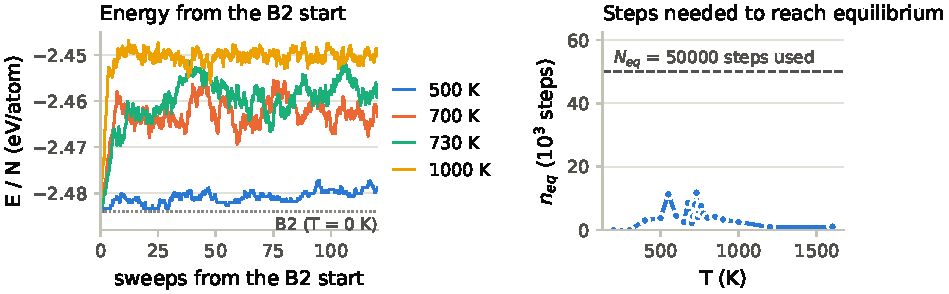
\includegraphics[width=\textwidth]{equilibration.pdf}
  \caption{Equilibration from the perfect B2 structure.
    Left: energy per atom during the first 120 sweeps at four temperatures (one value every 50 steps); the dotted line is the B2 energy.
    Right: number of steps $n_\mathrm{eq}$ needed to reach equilibrium at each temperature of the scan (first step with $E\ge E_\mathrm{eq}-\sigma$, see text); the dashed line is the number of steps $N_\mathrm{eq}=\num{50000}$ discarded in all the runs.}
  \label{fig:equilibration}
\end{figure}

At low temperature (200--300~K) the B2 structure is already the equilibrium state and almost no exchange is accepted.
At high temperature, disorder sets in within a few thousand steps.
The slowest relaxations are found below and near the transition, with at most \num{11806}~steps (27~sweeps) at \SI{730}{K}.
This estimate is itself noisy, because the energy fluctuates strongly near $\Tc$.
We therefore discard $N_\mathrm{eq}=\num{50000}$ steps at every temperature, more than four times the slowest relaxation.

% =====================================================================
\section{Physical quantities versus temperature}
\label{sec:results}

\Cref{fig:snapshots} shows what the configurations look like.
At \SI{300}{K} the layer is a perfect checkerboard of Cu and Zn.
Near $\Tc$ the order is only partial, and at \SI{1200}{K} the atoms are spread at random over the two sublattices.

\begin{figure}[ht]
  \centering
  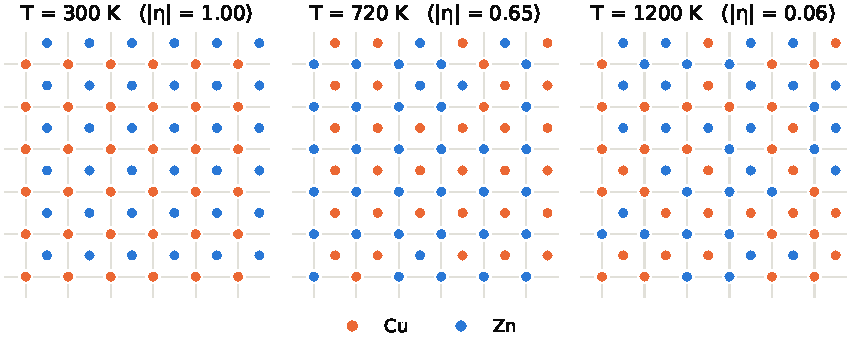
\includegraphics[width=\textwidth]{snapshots.pdf}
  \caption{Final configuration of the runs at three temperatures, seen from above: one layer of the box, with the $\alpha$ sites of height $z=0$ at the grid nodes and the $\beta$ sites of height $z=a/2$ at the centres of the squares ($6\times6$ cells, 72 of the 432 atoms). $|\eta|$ is computed on the whole box.}
  \label{fig:snapshots}
\end{figure}

\paragraph{Energy and heat capacity.}
The mean energy (\cref{fig:energy}, left) starts from the B2 value and rises steeply between 600 and \SI{800}{K}, where most of the disorder appears.
At high temperature it tends towards the energy of the ideal random alloy, $E_\mathrm{dis}/N = 4\bar J + 3\bar I = \SI{-2.4455}{eV/atom}$, where $\bar J$ and $\bar I$ are the averages of the pair energies weighted by the probabilities $\frac14,\frac14,\frac12$ of Cu--Cu, Zn--Zn and Cu--Zn pairs.
Even at \SI{1600}{K} the energy remains \SI{0.0023}{eV/atom} below this value, because of the short-range order discussed below.
The heat capacity (\cref{fig:energy}, right) has a clear peak at \SI{720}{K}; its value at \SI{700}{K} is almost the same, so the top of the peak is between 700 and \SI{720}{K}.

\begin{figure}[ht]
  \centering
  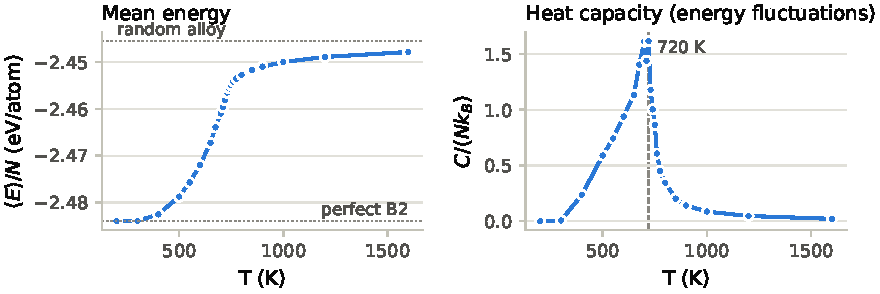
\includegraphics[width=\textwidth]{energy_heat.pdf}
  \caption{Left: mean energy per atom versus temperature; the dotted lines are the perfect B2 energy ($-2.484$~eV/atom) and the energy of an ideal random alloy ($-2.4455$~eV/atom).
    Right: heat capacity per atom in units of $k_B$, from the energy fluctuations (\cref{eq:fluctuations}); the dashed line marks its maximum.}
  \label{fig:energy}
\end{figure}

\paragraph{Long-range order.}
$\langle|\eta|\rangle$ (\cref{fig:order}, left) decreases slowly up to about \SI{600}{K}, then drops fast between 650 and \SI{800}{K}, and finally reaches the finite-size floor of the random lattice.
In an infinite crystal $\eta$ would vanish exactly at $\Tc$; in our small box the drop is rounded.
The susceptibility (\cref{fig:order}, right) has a sharp peak at \SI{720}{K}, almost equal to its value at \SI{730}{K}.

\begin{figure}[ht]
  \centering
  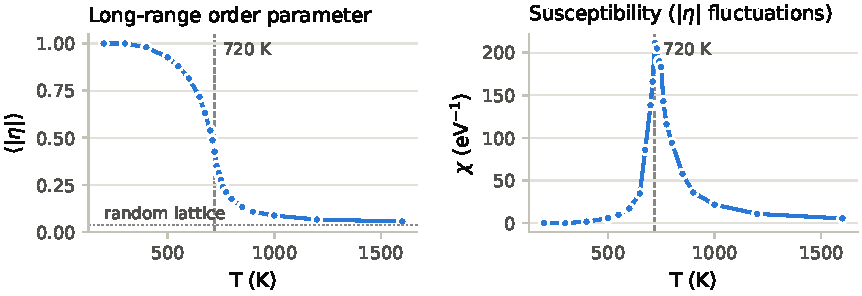
\includegraphics[width=\textwidth]{order_chi.pdf}
  \caption{Left: mean absolute long-range order parameter; the dotted line is the value for random lattices (finite-size floor), the dashed line marks the steepest drop.
    Right: susceptibility of the order parameter from the fluctuations of $|\eta|$ (\cref{eq:fluctuations}); the dashed line marks its maximum.}
  \label{fig:order}
\end{figure}

\Cref{fig:hist} explains these peaks.
Below $\Tc$ the distribution of $|\eta|$ is narrow around a large value; above $\Tc$ it is narrow close to zero.
Near $\Tc$ it is very broad: the system wanders between ordered and disordered states, so the fluctuations of $\eta$ and of $E$ are the largest there.

\begin{figure}[ht]
  \centering
  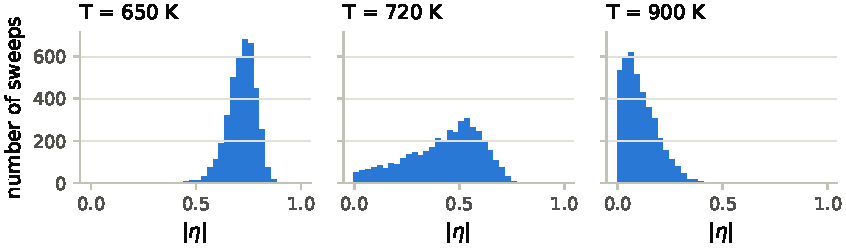
\includegraphics[width=\textwidth]{eta_hist.pdf}
  \caption{Histograms of the 4000 values of $|\eta|$ measured (one per sweep) below, near and above the transition. In our box $|\eta|$ can only take the values $2k/216$; each bin contains three of them (width $6/216\approx0.028$).}
  \label{fig:hist}
\end{figure}

\paragraph{Short-range order.}
\Cref{fig:cowley} shows the Cowley parameters.
If the only order were the long-range order, a Cu atom on $\alpha$ would find a Zn neighbour on $\beta$ with probability $(1+\eta)/2$, and a Cu atom on $\beta$ with probability $(1-\eta)/2$.
Averaging over the two cases gives $\alpha_1=-\eta^2$ and $\alpha_2=+\eta^2$ (dashed lines).
Below $\Tc$ the Cowley parameters follow these curves: the long-range order explains almost all the local order.
Above $\Tc$, however, $\langle\eta^2\rangle$ is almost zero while $\alpha_1$ stays clearly negative: at \SI{800}{K}, $\langle\alpha_1\rangle = -0.20$ whereas $-\langle\eta^2\rangle = -0.05$, and at \SI{1600}{K} $\langle\alpha_1\rangle$ is still $-0.07$.
Cu atoms keep more Zn first neighbours than in a random alloy: this \emph{short-range order} survives the loss of long-range order and fades slowly with temperature, as observed experimentally in ordering alloys~\cite{Moss1964}.

\begin{figure}[ht]
  \centering
  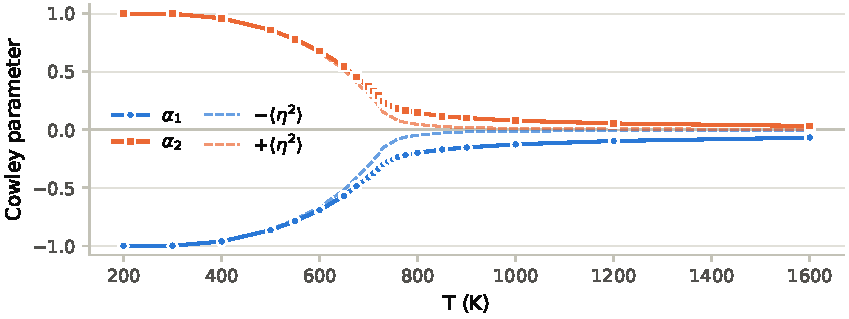
\includegraphics[width=\textwidth]{cowley.pdf}
  \caption{Cowley short-range order parameters for the first ($\alpha_1$, circles) and second ($\alpha_2$, squares) neighbour shells.
    The dashed lines $\mp\langle\eta^2\rangle$ are the values expected if the long-range order alone were present.
    The difference between symbols and dashed lines above \SI{750}{K} is the short-range order.}
  \label{fig:cowley}
\end{figure}

% =====================================================================
\section{Transition temperature}
\label{sec:tc}

We estimate $\Tc$ in three ways (\cref{tab:tc}): the maximum of the heat capacity, the maximum of the susceptibility, and the temperature where $\langle|\eta|\rangle$ drops the fastest (minimum of $\mathrm{d}\langle|\eta|\rangle/\mathrm{d}T$, by finite differences).
The three methods give the same grid temperature, \SI{720}{K}.
The grid step is \SI{10}{K} there, but the peaks are flat at the top, between 700 and \SI{730}{K} (\cref{tab:full}): we retain $\Tc \approx \SI{720}{K}$.

\begin{table}[!ht]
  \centering
  \caption{Transition temperature. The Monte Carlo values are read on the temperature grid of \cref{tab:conditions} (step \SI{10}{K} between 700 and \SI{760}{K}). The mean-field value is the Bragg--Williams approximation applied to the same pair model (see text).}
  \label{tab:tc}
  \begin{tabular}{lc}
    \toprule
    Method & $\Tc$ (K) \\
    \midrule
    Maximum of the heat capacity $C$ & 720 \\
    Maximum of the susceptibility $\chi$ & 720 \\
    Steepest drop of $\langle|\eta|\rangle$ & 720 \\
    \midrule
    Bragg--Williams mean field, same model & 894 \\
    Experiment ($\beta$-brass)~\cite{NixShockley1938,Massalski1990,KhanEisenbach2016} & $\approx 740$--$750$ \\
    \bottomrule
  \end{tabular}
\end{table}

\paragraph{Comparison with mean field.}
The Bragg--Williams approximation~\cite{BraggWilliams1934} keeps the long-range order $\eta$ but treats the atoms of each sublattice as independent.
The energy then reads $E/N = E_\mathrm{dis}/N - \Delta E\,\eta^2$, with $\Delta E = (E_\mathrm{dis}-E_\mathrm{B2})/N = \SI{0.0385}{eV/atom}$, and the entropy per atom is that of the random filling of each sublattice, $s \approx k_B(\ln 2 - \eta^2/2)$ for small $\eta$.
The free energy $E/N - Ts$ develops a minimum at $\eta\neq0$ below $k_B\Tc = 2\Delta E$, that is $\Tc^\mathrm{MF} = \SI{894}{K}$.
Our Monte Carlo value is about 20\,\% lower.
The difference comes from the short-range order seen in \cref{fig:cowley}: above $\Tc$ the atoms can lower their energy by local arrangements without any long-range order, which mean field ignores.
The disordered phase is therefore more stable than in mean field, and the transition happens at lower temperature.

% =====================================================================
\section{Discussion}
\label{sec:discussion}

\paragraph{Agreement with experiment.}
Our estimates of $\Tc$ are close to the experimental value, which is quite good for a model with only six parameters and no adjustment.
This agreement should not be over-interpreted: the model ignores the vibrations of the atoms, the thermal expansion of the lattice and the difference in size between Cu and Zn, and its pair energies are simple numbers.
For comparison, a rigid-lattice Monte Carlo study of CuZn with energies computed from first principles finds $\Tc\approx\SI{870}{K}$, about \SI{120}{K} above experiment~\cite{KhanEisenbach2016}: a good $\Tc$ is not a proof that every ingredient of the model is right.

\paragraph{Finite size.}
With $L=6$ the transition is rounded: $\langle|\eta|\rangle$ decreases continuously instead of vanishing at $\Tc$, never goes below the floor of \num{0.04}, and the peaks of $C$ and $\chi$ have a finite height and width.
The three estimators agree here, but they could differ by a few tens of kelvins: with only 800 sweeps per temperature, a first version of our analysis gave 700, 720 and \SI{730}{K}. The position of the peaks also depends on $L$.
A finite-size study with several box sizes (for example with the crossing of the Binder cumulant) would give $\Tc$ for an infinite crystal~\cite{LandauBinder2014,BinderHeermann2019}.

\paragraph{Sampling near $\Tc$.}
Successive measurements are correlated, especially near $\Tc$ where the order changes slowly (critical slowing down~\cite{NewmanBarkema1999}).
The heat capacity and the susceptibility are the noisiest quantities, because they are variances of correlated series; longer runs near $\Tc$ would make their peaks smoother.

\paragraph{Algorithm.}
Exchanging only first neighbours is a local dynamics that conserves the composition.
It satisfies detailed balance, so it samples the correct equilibrium distribution, but it is slow to move order over long distances.
Exchanges between any two sites would equilibrate faster at the same cost per step.

% =====================================================================
\section{Conclusion}

We wrote and tested a Metropolis Monte Carlo code for the order--disorder transition of CuZn on a rigid bcc lattice.
The tests on the perfect B2 structure and on random lattices give the expected values, and the energy updated move by move stays exact.
The cohesive energy of the B2 phase is \SI{2.484}{eV/atom}.
Starting from B2, the system needs at most about \num{12000} steps to reach equilibrium, so we discarded \num{50000} steps before measuring during \num{4000} sweeps.
The energy, the heat capacity, the long-range order parameter and its susceptibility all show the transition at $\Tc \approx \SI{720}{K}$, close to the experimental value (about \SI{740}{K}) and lower than the mean-field prediction (\SI{894}{K}).
Above the transition, Cu and Zn still prefer to be first neighbours: this short-range order explains why mean field overestimates $\Tc$.
The main limits of this study are the small size of the box and the simple pair model; larger boxes and a finite-size analysis would be the next step.

\printbibliography[heading=bibintoc, title={References}]

% =====================================================================
\clearpage
\appendix
\section{Full results of the temperature scan}
\label{app:table}

\begin{table}[ht]
  \centering
  \caption{Results of the temperature scan (conditions of \cref{tab:conditions}).
    $E$: mean energy per atom (eV); $C/(Nk_B)$: heat capacity per atom; $\chi$: susceptibility (\si{eV^{-1}}).}
  \label{tab:full}
  \small
  \begin{tabular}{rllllll}
\toprule
$T$ (K) & $\langle E\rangle/N$ & $C/(Nk_B)$ & $\langle|\eta|\rangle$ & $\chi$ & $\langle\alpha_1\rangle$ & $\langle\alpha_2\rangle$ \\
\midrule
200 & $-$2.4840 & 0.00 & 1.000 & 0 & $-$1.000 & 1.000 \\
300 & $-$2.4840 & 0.01 & 1.000 & 0 & $-$1.000 & 1.000 \\
400 & $-$2.4825 & 0.24 & 0.980 & 2 & $-$0.962 & 0.961 \\
500 & $-$2.4788 & 0.59 & 0.926 & 6 & $-$0.865 & 0.861 \\
550 & $-$2.4757 & 0.74 & 0.879 & 10 & $-$0.787 & 0.779 \\
600 & $-$2.4720 & 0.94 & 0.815 & 17 & $-$0.692 & 0.678 \\
650 & $-$2.4673 & 1.13 & 0.717 & 35 & $-$0.570 & 0.547 \\
675 & $-$2.4639 & 1.40 & 0.631 & 86 & $-$0.485 & 0.455 \\
700 & $-$2.4610 & 1.61 & 0.539 & 139 & $-$0.409 & 0.373 \\
710 & $-$2.4596 & 1.44 & 0.487 & 166 & $-$0.374 & 0.335 \\
720 & $-$2.4582 & 1.62 & 0.427 & 211 & $-$0.337 & 0.295 \\
730 & $-$2.4565 & 1.18 & 0.350 & 205 & $-$0.296 & 0.249 \\
740 & $-$2.4556 & 1.00 & 0.313 & 190 & $-$0.272 & 0.224 \\
750 & $-$2.4549 & 0.86 & 0.276 & 183 & $-$0.254 & 0.205 \\
760 & $-$2.4542 & 0.61 & 0.240 & 143 & $-$0.235 & 0.185 \\
775 & $-$2.4535 & 0.45 & 0.212 & 116 & $-$0.218 & 0.167 \\
800 & $-$2.4528 & 0.34 & 0.176 & 94 & $-$0.199 & 0.146 \\
850 & $-$2.4517 & 0.20 & 0.133 & 58 & $-$0.170 & 0.117 \\
900 & $-$2.4510 & 0.14 & 0.108 & 36 & $-$0.152 & 0.101 \\
1000 & $-$2.4500 & 0.09 & 0.088 & 22 & $-$0.126 & 0.078 \\
1200 & $-$2.4489 & 0.05 & 0.067 & 11 & $-$0.097 & 0.054 \\
1600 & $-$2.4478 & 0.02 & 0.056 & 5 & $-$0.068 & 0.033 \\
\bottomrule
\end{tabular}

\end{table}

\section{Code and reproduction}
\label{app:code}

The model is written in Python in \texttt{src/model.py} (one module, about 190 lines):
\begin{itemize}\setlength{\itemsep}{0pt}
  \item the array \texttt{sous\_reseau} holds the species of each site (0 = Cu, 1 = Zn); site $i$ of cell $(x,y,z)$ and sublattice $s$ has index $i = 2(x+6y+36z)+s$, so even sites are $\alpha$ and odd sites $\beta$;
  \item \texttt{FIRST\_NEIGHBOURS} and \texttt{SECOND\_NEIGHBOURS} are the neighbour tables, built once at import;
  \item \texttt{get\_full\_energy()} computes \cref{eq:energy}; \texttt{energy\_after\_flip(E, i, j)} returns the energy after exchanging $i$ and $j$ from the local bonds only, without changing the configuration; \texttt{flipping\_proba} and \texttt{flipping\_action} apply the Metropolis rule;
  \item \texttt{cowley()} and \texttt{order\_parameter()} return $(\alpha_1,\alpha_2)$ and $\eta$;
  \item \texttt{metropolis\_before\_eq(n, T)} returns the energy after each of $n$ steps from B2 (equilibration test); \texttt{metropolis(n\_eq, n\_meas, T, measure\_every)} returns the series of $E$, $|\eta|$, $\alpha_1$, $\alpha_2$ measured after equilibration.
\end{itemize}
The analysis notebook \texttt{analysis.ipynb} uses these functions interactively.
All the figures and tables of this report are produced by \texttt{report/make\_figures.py}, with the parameters of \cref{tab:conditions}.
From the project folder:
\begin{verbatim}
python -m venv .venv && .venv/bin/pip install -r requirements.txt
.venv/bin/python -B report/make_figures.py --rerun   # simulations, figures
cd report && latexmk -pdf report.tex slides.tex       # report and slides
\end{verbatim}

\end{document}
